\documentclass[a4paper,10pt]{book}

\usepackage{latexsym}
\usepackage{graphicx}
\usepackage{supertabular}
\usepackage{xspace}
\usepackage{pdfpages}
\usepackage{hyperref} 
\usepackage{listings}
\usepackage{color} 
\usepackage{colortbl}
\usepackage{ctable}
\usepackage{enumitem}

\usepackage[cc]{titlepic}
\usepackage{sectsty}
\usepackage[T1]{fontenc}
\usepackage[urw-garamond]{mathdesign}
\usepackage{fncychap}
\usepackage{fancyhdr}
\usepackage{lscape}

\usepackage{dirtree}
\usepackage{tikz}
\usetikzlibrary{arrows, shapes, positioning}
\usepackage{adjustbox}

\usepackage{rail}
\railoptions{-t -h}

\fancyhead{} % clear all header fields
\fancyheadoffset[LE,RO]{\marginparsep+\marginparwidth}
\fancyhead[RO,LE]{\thepage}
\fancyhead[LO]{\rightmark}
\fancyhead[RE]{\leftmark}
\renewcommand{\headrulewidth}{0.1pt}

\fancyfoot{}


\hypersetup{%
            colorlinks = true, %true, false
            linkcolor = black,
            citecolor = blue,
            urlcolor = blue,
}
\urlstyle{sf} %rm
\newcommand{\myurl}[1]{\textcolor{blue}{\underbar{\url{#1}}}}


%%%%%%%%%%%%%%%%%%%command imported from lac paper
\newcommand{\code}[1]	{\lstinline'#1'}
\newcommand{\OSTab}[1]	{\multicolumn{3}{|l|}{\hspace{14mm}\emph{#1}}}
\newcommand{\htab}		{\hspace*{3mm}}

\newcommand{\ros}		{\textsc{ROS}\xspace}

\newcommand{\faust}		{\textsc{Faust}\xspace}
\newcommand{\grame}		{\textsc{Grame}\xspace}
\newcommand{\cierec}	{\textsc{Cierec}\xspace}
\newcommand{\ccrma}		{\textsc{Ccrma}\xspace}
\newcommand{\cnmat}		{\textsc{Cnmat}\xspace}
\newcommand{\create}	{\textsc{Create}\xspace}
\newcommand{\mines}		{\textsc{Mines} ParisTech\xspace}
\newcommand{\pdf}		{\textsc{Pdf}\xspace}
\newcommand{\ie}		{i.e.\ }


%%%%%%%%%%%%%%%%%%%%%%%%%%%%%%%%%%%%%%%%%%%%%%%%%


%%% MY COLORS
\definecolor{yoheader}{rgb}{0.71,0.01,0.0}

\definecolor{darkcerulean}{rgb}{0.03, 0.27, 0.49}
\definecolor{darkpastelblue}{rgb}{0.47, 0.62, 0.8}
\definecolor{indigodye}{rgb}{0.0, 0.25, 0.42}

\definecolor{roscolor}{HTML}{1F2A44}
\definecolor{faustcolor}{HTML}{E76E18}


%%%% margin par
\definecolor{margincolor}{rgb}{0.52,0.02,0.02} % grey red.
\definecolor{yobg}{rgb}{0.9,0.9,1}
\definecolor{yotxt}{rgb}{0.01,0.01,0.52}
\definecolor{mylstcmt}{rgb}{0.01,0.52,0.01} % a dark green..
\definecolor{mylstdoc}{rgb}{0.80,0.30,0.80} % a medium pink.
\definecolor{mylstkey}{rgb}{0.52,0.01,0.01} % a dark red.

\setlength{\marginparwidth}{1.2in}
\let\oldmarginpar\marginpar
\renewcommand\marginpar[1]{\-\oldmarginpar[\raggedleft\color{margincolor}\footnotesize #1]%
{\raggedright\color{margincolor}\footnotesize #1}}



% \relax

\begin{document} 

\ChRuleWidth{1pt}
\ChNumVar{\raggedleft\Huge\color{yoheader}}
\ChTitleVar{\raggedleft\sffamily\fontsize{30}{32}\bf\color{yoheader}}

\chapterfont{\color{yoheader}}
\sectionfont{\color{yoheader}}
\subsectionfont{\color{yoheader}}
\subsubsectionfont{\color{yoheader}}

% parameters for listings
\lstset{
  tabsize=4,
  showspaces=false,
  showstringspaces=false,
  language=C++, 
  basicstyle=\ttfamily\color{yotxt},
  numbers=none,
  stepnumber=2,
  commentstyle=\slshape\color{mylstcmt},
  breaklines=true, 
  emph={component, declare, environment, import, library, process},
  emph={[2]ffunction, fconstant, fvariable},
  emph={[3]button, checkbox, vslider, hslider, nentry, vgroup, hgroup, tgroup, vbargraph, hbargraph, attach},
  emphstyle=\color{mylstkey},
  morecomment=[s][\color{mylstdoc}]{<mdoc>}{</mdoc>},
  backgroundcolor=\color{yobg},
  captionpos=b
}

\lstloadlanguages{C++,[LaTeX]TeX}

\title{\Huge\color{yoheader}Using FAUST with ROS\\\Large(version 0.0.09)}
\author{\textsc{Grame}\\Centre National de Cr\'eation Musicale}
\date{December 2014} 


\railalias{recur}{$\sim$}
\railalias{lbrace}{\{}
\railalias{rbrace}{\}}
\railalias{dollar}{\$}
\railalias{mod}{\%}
\railalias{arobase}{@}
\railalias{ampersand}{\&}
\railalias{hat}{$\land$}
\railalias{kot}{'}
\railalias{pipe}{$|$}
\railalias{fdelay}{}
\railalias{backslash}{\char"5C}
\railterm{recur,lbrace,rbrace,dollar,mod,kot,arobase,ampersand,backslash,fdelay, pipe, hat}

\newcommand{\farg}[1]{\textrm{\textit{#1}}}
\newcommand{\ldbrack}{[\![ \,}
\newcommand{\rdbrack}{\, ]\!] }
\newcommand{\rdbrackC}{\rdbrack_{\mathrm{C}}\,}
\newcommand{\dbrack}[1]{\ldbrack #1 \rdbrack}
\newcommand{\semantic}[1]{\ldbrack #1 \rdbrack}
\newcommand{\dbrackC}[1]{\ldbrack #1 \rdbrackC}

\newcommand{\latex}{\LaTeX\xspace}
\newcommand{\ircam}{\textsc{Ircam}\xspace}
\newcommand{\astree}{\textsc{Astree}\xspace}
\newcommand{\svg}{\textsc{Svg}\xspace}
 

\setlength{\parindent}{0pt}
\setlength{\parskip}{1ex plus 0.5ex minus 0.2ex}

\maketitle

\tableofcontents


%%%%%%%%%%%%%%%%%%%%%%%%%%%%%%%%%%%%%%%%%%%%%%%%%%%%%%%%%%%%%%%%%%%%%%%%%%%%%%%%%%%%%%
%%%%%%%%%%%%%%%%%%%%%%%%%%%%%%%%%%%%%%%%%%%%%%%%%%%%%%%%%%%%%%%%%%%%%%%%%%%%%%%%%%%%%%
%                            		CHAPTERS                                        %
%%%%%%%%%%%%%%%%%%%%%%%%%%%%%%%%%%%%%%%%%%%%%%%%%%%%%%%%%%%%%%%%%%%%%%%%%%%%%%%%%%%%%%
%%%%%%%%%%%%%%%%%%%%%%%%%%%%%%%%%%%%%%%%%%%%%%%%%%%%%%%%%%%%%%%%%%%%%%%%%%%%%%%%%%%%%%

\chapter{Introduction}
\label{chap:intro}

\faust (\textit{Functional Audio Stream}) is a functional programming language specifically designed for real-time signal processing and synthesis.  \faust targets high-performance signal processing applications and audio plug-ins for a variety of platforms and standards.\newline
\ros (\textit{Robot Operating System}) is a flexible framework for writing robot software. It is a collection of tools, libraries, and conventions that aim to simplify the task of creating complex and robust robot behavior across a wide variety of robotic platforms.


\section{\faust} 
\subsection{Design Principles}

Various principles have guided the design of \faust :

\begin{itemize}

\item \faust is a \textit{specification language}. It aims at providing an adequate notation to describe \textit{signal processors} from a mathematical point of view. \faust is, as much as possible, free from implementation details. 

\item \faust programs are fully compiled, not interpreted. The compiler translates \faust programs into equivalent C++ programs taking care of generating the most efficient code. The result can generally compete with, and sometimes even outperform, C++ code written by seasoned programmers. 

\item The generated code works at the sample level. It is therefore suited to implement low-level DSP functions like recursive filters. Moreover the code can be easily embedded. It is self-contained and doesn't depend of any DSP library or runtime system. It has a very deterministic behavior and a constant memory footprint. 

\item The semantic of \faust is simple and well defined. This is not just of academic interest. It allows the \faust compiler to be \emph{semantically driven}. Instead of compiling a program literally, it compiles the mathematical function it denotes. This feature is useful for example to promote components reuse while preserving optimal performance.  

\item \faust is a textual language but nevertheless block-diagram oriented. It actually combines two approaches: \textit{functional programming} and \textit{algebraic block-diagrams}. The key idea is to view block-diagram construction as function composition. For that purpose, \faust relies on a \emph{block-diagram algebra} of five composition operations (\lstinline': , ~ <: :>').

\item Thanks to the notion of \textit{architecture}, \faust programs can be easily deployed on a large variety of audio platforms and plugin formats without any change to the \faust code.

\end{itemize}

\subsection{Signal Processor Semantic}
A \faust program describes a \emph{signal processor}. 
The role of a \textit{signal processor} is to transform a group  of (possibly empty) \emph{input signals} in order to produce a group of (possibly empty) \emph{output signals}. 
Most audio equipments can be modeled as \emph{signal processors}. 
They have audio inputs, audio outputs as well as control signals interfaced with sliders, knobs, vu-meters, etc... \\

For more informations about \faust, please see \textit{faust-quick-reference.pdf} and the tutorials in \faust documentation.

\section{\ros}
\subsection{What is it ?}
\marginpar {This section's content (1.2 \ros) is taken from \ros documentation. It can be found on \href{http://www.ros.org}{\ros official website} and \href{http://www.wiki.ros.org }{\ros wiki}.} Creating truly robust, general-purpose robot software is \textit {hard}. From the robot's perspective, problems that seem trivial to humans often vary wildly between instances of tasks and environments. Dealing with these variations is so hard that no single individual, laboratory, or institution can hope to do it on their own. \newline

\ros is an open-source, meta-operating system for your robot. It provides the services you would expect from an operating system, including hardware abstraction, low-level device control, implementation of commonly-used functionality, message-passing between processes, and package management. It also provides tools and libraries for obtaining, building, writing, and running code across multiple computers. \newline

As a result, \ros was built from the ground up to encourage \textit{collaborative} robotics software development. For example, one laboratory might have experts in mapping indoor environments, and could contribute a world-class system for producing maps. Another group might have experts at using maps to navigate, and yet another group might have discovered a computer vision approach that works well for recognizing small objects in clutter. \ros was designed specifically for groups like these to collaborate and build upon each other's work, as is described throughout this site.\\

\subsection{Concepts}
\subsubsection{Filesystem level}
The filesystem level concepts mainly cover \ros resources that you encounter on disk, such as:

\begin{itemize}

\item \textbf{Packages} are the main unit for organizing software in \ros. 
	A package may contain \ros runtime processes (nodes), a \ros-dependent library, datasets, configuration files, or anything else that is usefully organized together. 
	Packages are the most atomic build item and release item in \ros. Meaning that the most granular thing you can build and release is a package.

\item \textbf{Metapackages} are specialized Packages which only serve to represent a group of related other packages. 


\item \textbf{Services : }
Service descriptions, stored in my\_package/srv/MyServiceType.srv, define the request and response data structures for  \href{http://wiki.ros.org/Services}{services} in \ros.

\item \textbf{Messages : }  
Message descriptions, stored in my\_package/msg/MyMessageType.msg, define the data structures for  \href{http://wiki.ros.org/Messages}{messages} sent in \ros.


\end{itemize}


\subsubsection{Computation Graph level}
The Computation Graph is the peer-to-peer network of \ros processes that are processing data together. The basic Computation Graph concepts of \ros are nodes, Master, Parameter Server, messages, services, topics, and bags, all of which provide data to the Graph in different ways.

\begin{itemize}
\item \textbf{Master : }
The \ros Master provides name registration and lookup to the rest of the Computation Graph. Without the Master, nodes would not be able to find each other, exchange messages, or invoke services.

\item \textbf{Nodes : } 
Nodes are processes that perform computation. \ros is designed to be modular at a fine-grained scale; a robot control system usually comprises many nodes. For example, one node controls a laser range-finder, one node controls the wheel motors, one node performs localization, one node performs path planning, one Node provides a graphical view of the system, and so on. A \ros node is written with the use of a \ros client \href{http://wiki.ros.org/Client\%20Libraries}{library}, such as \href{http://wiki.ros.org/roscpp}{roscpp} or \href{http://wiki.ros.org/rospy}{rospy}.

\item \textbf{Topics : } Messages are routed via a transport system with publish / subscribe semantics. A node sends out a message by publishing it to a given \href{http://wiki.ros.org/Topics}{topic}. The topic is a name that is used to identify the content of the message. A node that is interested in a certain kind of data will subscribe to the appropriate topic. There may be multiple concurrent publishers and subscribers for a single topic, and a single node may publish and/or subscribe to multiple topics. In general, publishers and subscribers are not aware of each others' existence. The idea is to decouple the production of information from its consumption. Logically, one can think of a topic as a strongly typed message bus. Each bus has a name, and anyone can connect to the bus to send or receive messages as long as they are the right type.

\item \textbf{The Parameter Server : }The Parameter Server allows data to be stored by key in a central location. It is currently part of the Master.

\item \textbf{Messages : }Nodes communicate with each other by passing \href{http://wiki.ros.org/Messages}{messages}. A message is simply a data structure, comprising typed fields. Standard primitive types (integer, floating point, boolean, etc.) are supported, as are arrays of primitive types. Messages can include arbitrarily nested structures and arrays (much like C structures).

\end{itemize}

\begin{figure}[ht!]
\centering

 \begin{tikzpicture} [remember picture]
 \node[draw=teal, label={[teal] above left:{MASTER}}, ] (master) {
 	\begin{tikzpicture}[node distance=2cm]
	  \node[draw, fill=cyan, ellipse, text width=1.5cm, align=center](n1){Node 1};	  
	  \node[draw, fill=cyan, ellipse, text width=1.5cm, below=of n1, align=center](n2){Node 2};
	  \node[draw, fill=orange, rounded corners=3pt, text width=1.5cm, right=of n1, align=center](t1){Topic 1};
	  \node[draw, fill=orange, rounded corners=3pt, text width=1.5cm, right=of n2, align=center](t2){Topic 2};
	  \node[draw, fill=cyan, ellipse, text width=1.5cm, right=of t1, align=center](n3){Node 3};
	  \node[draw, fill=cyan, ellipse, text width=1.5cm, below=of n3, align=center](n4){Node 4};
	  
 
	  \draw[margincolor,->, very thick] (n1) to node [sloped, midway, above] {publishing} (t1);
	  \draw[margincolor,->, very thick] (n2) to node [sloped, midway, above] {publishing} (t1.south west);
 	  \draw[margincolor,->, very thick] (n3) to node [sloped, midway, above] {publishing} (t2.north east);
	  \draw[yoheader,->, very thick] (t1) to node [sloped, midway, above] {subscribing} (n3);
 	  \draw[yoheader,->, very thick] (t2) to node [sloped, midway, above] {subscribing} (n2);
  	  \draw[yoheader,->, very thick] (t2) to node [sloped, midway, above] {subscribing} (n4);
	\end{tikzpicture}
 };
  
 \end{tikzpicture}

\caption{\ros Concepts in a Diagram }
\label{fig:ROS Concepts}
\end{figure}

\subsubsection{Names}
Names are really important in \ros. Valid names have these characteristics :
\begin{itemize}
	\item first chararacter is an alpha character : [a-z][A-Z]
	\item subsequent characters can be alphanumeric : [a-z][A-Z][0-9], underscores : \_ or forward slash : /
	\item there is at most one forward slash : /

\end{itemize}

For more informations on \ros and tutorials, please have a look to the website :
\myurl{www.wiki.ros.org}.\\
\newpage
\section{Using \faust with \ros}
The idea of using \faust modules with \ros could be summed up in the following diagrams.

\begin{figure}[ht!]
\centering

\begin{tikzpicture} [remember picture, node distance=0.5cm]
 \node[draw, dashed, label=above:{\faust part}] (faust) {
 	\begin{tikzpicture}
	 \node[draw, solid, text=yoheader, fill=lightgray] (dsp) {.dsp file};
	 \node[draw=yoheader, solid, ellipse, text=black, right=of dsp, text width=1.5cm, align=center](compiler) {\faust compiler};
	 \draw[->, very thick, solid] (dsp)--(compiler);
	 \end{tikzpicture}
 };
 \node[draw, dashed, right=of faust, label=above:{\ros part}] (ROS) {
	 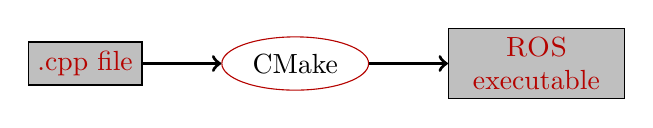
\begin{tikzpicture}
	 \node[draw, solid, text=yoheader, fill=lightgray] (cpp) {.cpp file};
	 \node[draw=yoheader, solid, ellipse, text=black, right=of cpp] (CMake) {CMake};
	 \node[draw, solid, text=yoheader, fill=lightgray, right=of CMake, text width=2cm, align=center] (exec) {\ros executable};
	 \draw[->, very thick, solid] (cpp)--(CMake);
	 \draw[->, very thick, solid] (CMake)--(exec);
	 \end{tikzpicture}
 };
 \draw[->,very thick] (compiler.east) -- (cpp.west);
 
\end{tikzpicture}
\caption{Compilation process }
\label{fig:Compilation principle}
\end{figure}

As shown on figure~\ref{fig:Compilation principle}, the dsp file is compiled into a C++ file thanks to the \faust compiler. Then, the C++ file can be compiled with CMake in a \ros package to create a \ros executable, that you can run with \lstinline'rosrun'.

\begin{figure}[ht!]
\centering

 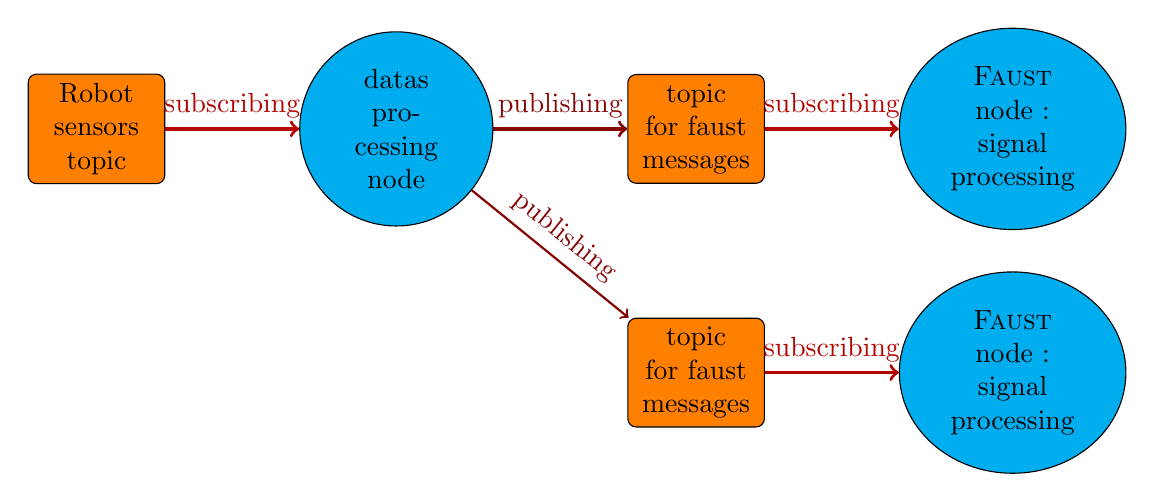
\begin{tikzpicture} [remember picture, node distance=1.7cm]
 
  \node[draw, fill=orange, rounded corners=3pt, text width=1.5cm, align=center](sensor topic){Robot sensors topic};
  \node[draw, fill=cyan, ellipse, text width=1.5cm, right=of sensor topic, align=center](process node){datas processing node};
  \node[draw, fill=orange, rounded corners=3pt, text width=1.5cm, align=center,  right=of process node](faust topic){topic for faust messages};
  \node[draw, fill=orange, rounded corners=3pt, text width=1.5cm, align=center,  below=of faust topic](faust topic2){topic for faust messages};
  \node[draw, fill=cyan, ellipse, text width=1.8cm, right=of faust topic, align=center](faust node){\faust node : signal processing};
 \node[draw, fill=cyan, ellipse, text width=1.8cm, right=of faust topic2, align=center](faust node2){\faust node : signal processing};
 
 \draw[yoheader,->, very thick] (sensor topic) to node [sloped, midway, above] {subscribing} (process node);
 \draw[margincolor,->, very thick] (process node) to node [sloped, midway, above] {publishing} (faust topic);
 \draw[margincolor,->, thick] (process node) to node [sloped, midway, above] {publishing} (faust topic2);
 \draw[yoheader,->, very thick] (faust topic) to node [sloped, midway, above] {subscribing} (faust node);
 \draw[yoheader,->, very thick] (faust topic2) to node [sloped, midway, above] {subscribing} (faust node2);
 
 \end{tikzpicture}

\caption{Robot using \ros}
\label{fig:Use Diagram}
\end{figure}

Once the executables coming from DSP files compiled, you can run and combine then with robotic applications (figure~\ref{fig:Use Diagram}).\\
\newpage
\section{Audio Server}
\faust applications use the jack audio server. Make sure it is installed on your machine.
\begin{figure}[ht!]
	\centering
	\begin{tikzpicture}[remember picture, node distance=3.5cm]
	
		\node[node distance=0, label=\color{teal}{Node 1}](node1)
		{
			\begin{tikzpicture}
				\node[draw=black,text=white, fill=indigodye, text width=4cm, align=center](processing1){\ros : processing \\ and interface};
				\node[draw=black, fill=darkpastelblue, below=of processing1, text width=4cm, align=center](audio1){jack : audio server};
			\end{tikzpicture}
		};
		\node[right=of node1, node distance=0, label=\color{teal}{Node 2}](node2){
			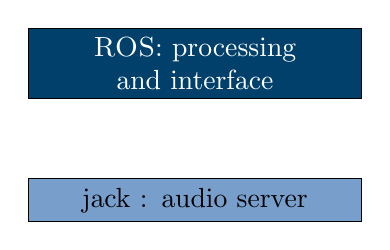
\begin{tikzpicture}
				\node[draw=black,text=white, fill=indigodye, text width=4cm, align=center](processing2){\ros : processing \\ and interface};
				\node[draw=black, fill=darkpastelblue, below=of processing2, text width=4cm, align=center](audio2){jack : audio server};
			\end{tikzpicture}		
		};	
		 \draw[indigodye, <->, very thick, text width=3cm, align=center] (processing1.east) to node [sloped, midway, above] {nodes parameters \\ through topics} (processing2.west);
		  \draw[darkpastelblue, <->, very thick] (audio1.east) to node [sloped, midway, below, darkcerulean] {audio datas} (audio2.west);

	\end{tikzpicture}
	
	\caption{APIs used by \faust nodes}
	\label{fig: Audio server}
\end{figure}
\chapter{Compiling \faust Program for \ros Use}
\label{chap:compilation}

To compile a \faust program for a \ros use, you can use either the \lstinline'faust2ros' command, or the \lstinline'faust2rosgtk' one, which adds a gtk graphic user interface to the simple \lstinline'faust2ros' command.
Note that all the \faust compilation options remain.

\section{Compiling in a \faust Archive}
In order to compile a DSP file into a \faust archive, just type the command followed by your file : 
\begin{lstlisting}
faust2ros file.dsp
\end{lstlisting}
It should output :
\begin{lstlisting}
file.zip;
\end{lstlisting}
and the resulting  \lstinline'file.zip' folder should contain the following elements:

\begin{tabular}{ll}
	\lstinline'faust_msgs' 		&messages package to handle faust messages\\
	\lstinline'file'		&package containing a .cpp file corresponding to the DSP file\\
\end{tabular}

If the DSP file is not in the current directory, make sure to type the right path. For instance :
\begin{lstlisting}
faust2ros ~/faust/examples/myfile.dsp
\end{lstlisting}


\paragraph{Comment:}If you want to use the \lstinline'faust2rosgtk' command, the output will have a \lstinline'_gtk' extension. For instance :
\begin{lstlisting}
faust2rosgtk file.dsp
\end{lstlisting}
should output :
\begin{lstlisting}
file_gtk.zip;
\end{lstlisting}
and the resulting  \lstinline'file_gtk.zip' folder should contain the following elements:

\begin{tabular}{ll}
	\lstinline'faust_msgs' 		&messages package to handle faust messages\\
	\lstinline'file_gtk'		&package containing a .cpp file corresponding to the DSP file\\
\end{tabular}

\section{Compiling in a Workspace}
Thanks to the option \lstinline'-install', you have the possibility to create a package from your DSP file directly in the a workspace you chose.
Just type :
\begin{lstlisting}
faust2ros -install faust_ws file.dsp
\end{lstlisting}

It should output : 
\begin{lstlisting}
file.cpp; 
\end{lstlisting}
and you should have a faust\_ws repository looking like this :\\

\dirtree{%
.1 faust\_ws. 
	.2 build. 
	.2 devel. 
	.2 src. 
		.3 faust\_msgs : \begin{minipage}[t]{10cm}
						Messages Package \\
						Files to handle \faust messages{.}
					   \end{minipage}. 
			.4 include. 
			.4 msg. 
				.5 param\_faust.msg. 
			.4 src. 
			.4 CMakeLists.txt. 
			.4 package.xml. 
		.3 file :  \begin{minipage}[t]{10cm}
						File Package
						{.}
				\end{minipage}.
			.4 include. 
			.4 src. 
				.5 \textcolor{margincolor}{file.cpp} : 
						\begin{minipage}[t]{10cm}
						File generated with \faust compiler
						{.}
					   \end{minipage}. 
			.4 CMakeLists.txt. 
			.4 package.xml. 
}

%\section{Renaming DSP file}
%If the dsp file name does not fit you, you can change it using the \lstinline'-o' command.
%For instance, if you want the package generated from DSP file to have a different name that your DSP file name, you can type :
%\begin{lstlisting}
%	faust2ros -o foobar file.dsp
%\end{lstlisting}
%The output is going to be : \\
%
%\dirtree{%
%.1 foobar.zip. 
%	.2 faust\_msgs. 
%	.2 foobar. 
%}
%\newpage
\section{Example}
Here is an example of three files compilation.\\

Input :
\begin{lstlisting}
faust2rosgtk -install foo_ws -o foo1 file1.dsp 
			 -install foo_ws -o foo2 file2.dsp 
			 -install bar_ws -o bar file3.dsp
\end{lstlisting}
\newpage
Output :\\
\dirtree{%
.1 \~{ }. 	
	.2 foo\_ws. 
		.3 faust\_msgs. 
		.3 foo1. 
		.3 foo2. 
	.2 bar\_ws. 
		.3 bar. 
}
\chapter{Using FAUST Nodes}
\label{chap:run}
Once your DSP files are compiled into \ros executables, you can run them into a \ros master.

\section{Run the Master}
A \faust node needs a master to run. You can check if a master is already running by typing :
\begin{lstlisting}
rostopic list
\end{lstlisting}
Then, there are two possibilities :
\begin{itemize}
	\item either you get the following message :
	\begin{lstlisting}
ERROR: Unable to communicate with master!
	\end{lstlisting}
	which means there is no master running
	\item or you get :
	\begin{lstlisting}
/rosout
/rosout_agg
	\end{lstlisting}
	which means a master is already running.
\end{itemize}
To run a master, you have to type the following command :
\begin{lstlisting}
roscore
\end{lstlisting}

\newpage
\section{Run a FAUST Node}
Now that your master is running, you can run your \faust node. It is quite simple. Type :
\begin{lstlisting}
rosrun mynodepackage mynode
\end{lstlisting}
For instance, if your node name is \textit{foo}, then type :
\begin{lstlisting}
rosrun foo foo
\end{lstlisting}
If you get an error message looking like this :
\begin{lstlisting}
[rosrun] Couldn't find executable named foo below /path/to/myworkspace/src/foo
\end{lstlisting}
then refer to section~\ref{sec:rosrun error}

\section{To Which Topics is a FAUST Node Subscribing ?}
Once your \faust node is running, it automatically subscribes to topics corresponding to the parameters you can modify, and to the widgets the gtk graphic interface has. For instance, if you use a \faust node generated from the noise.dsp file (in the examples directory), the noise\_gtk node will subscribe to the topic \lstinline'noise_gtk/Volume' and the graphic interface will look like this :
\begin{figure}[ht!]
\centering
\begin{adjustbox}{minipage=5cm,margin=0pt 10pt,bgcolor=roscolor}
\centering
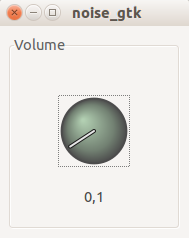
\includegraphics[scale=0.5]{images/noise_gtk.png}
\end{adjustbox}
\caption{noise\_gtk graphic interface}
\label{fig:noise_gtk}

\end{figure}
\newpage
A more complex example like the harpe.dsp file, which contains three widgets, can generate several topics to subscribe to :
\\
\begin{center}

\begin{tabular}{l}
	\lstinline'/harpe_gtk/attenuation' \\
	\lstinline'/harpe_gtk/hand' \\
	\lstinline'/harpe_gtk/level' \\
\end{tabular}\\
\end{center}
and the graphic interface can look like this :
\begin{figure}[ht!]
\centering
\begin{adjustbox}{minipage=5cm,margin=0pt 10pt,bgcolor=roscolor}
\centering
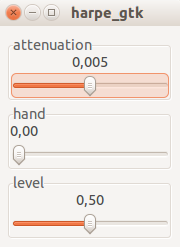
\includegraphics[scale=0.5]{images/harpe_gtk.png}
\end{adjustbox}
\caption{harpe\_gtk graphic interface}
\label{fig:harpe_gtk}
\end{figure}

If you want to change the topic name, just remap them while running your node :
\begin{lstlisting}
rosrun myfaustpackage myfaustnode /topicname:=/newtopicname
\end{lstlisting}
For instance, to remap the /harpe/hand topic to /play, then run the harpe node like this :
\begin{lstlisting}
rosrun harpe harpe /harpe/hand:=/play
\end{lstlisting}

\paragraph{Comment:}The \faust nodes subscribe to topics using std\_msgs message types. Depending on the widgets you use, you can subscribe to default topics using either Float32 or Bool messages.\\

\begin{center}
	\begin{tabular}{ | c | c | }
		\hline
		\rowcolor{yobg} Widget & Message type \\ \hline
		Button & std\_msgs/Bool \\ \hline
		Check Button & std\_msgs/Bool \\ \hline
		Slider & std\_msgs/Float32 \\ \hline
		Num. Entry & std\_msgs/Float32 \\ \hline
	\end{tabular}
\end{center}

\newpage

\section{How to Escape from a Running Node ?}
To close a node running in \ros, you have two possibilities, depending on the graphic interface :
\begin{itemize}
	\item If your node has a graphic interface, then quit by clicking on the red cross in the corner of the window.
	\item If your node does not have any graphic interface, then quit by typing Ctrl+C in the node's terminal window.
\end{itemize}
\chapter{Metadata}
\label{chap:spec}
You might not want to use the float or bool standard messages for your topic, and compile the dsp file directly with the right topic name. In order to accomplish this, you can use \ros metadata.
\section{DSP writing}
It all starts in the widgets definition. Until now, maybe that you only wrote :
\begin{lstlisting}
param = hslider("level", etc);
\end{lstlisting}
To use \ros metadata, you simply have to add square brackets with your topic parameters :
\begin{lstlisting}
param = hslider("level [ros:/my/topic/name msg_type msg_name field_name]", etc);
\end{lstlisting}
~\\
As an example, if you intend to use integers in a foo/bar/baz topic, you can type :
\begin{lstlisting}
param = hslider("level [foo/bar/baz std_msgs Int32 data]", etc);
\end{lstlisting}
And if you intend to use the y field of a Point32 geometry\_msg, then type :
\begin{lstlisting}
param = hslider("level [foo/bar/baz geometry_msgs Point32 y]", etc);
\end{lstlisting}
You can also add the minimal and maximal values of the signal (4.1 and 9.3 for instance) by adding in the metadata declaration :
\begin{lstlisting}
param = hslider("level [foo/bar/baz std_msgs Int32 data 4.1 9.3]", etc);
\end{lstlisting}
\paragraph{\color{yoheader}BE CAREFUL !}The minimal and maximal values must be floats ! Otherwise, compilation fails.
\newpage
\section{Compilation}
To compile your dsp file, just do like you used to do before to find out this wonderful chapter about metadata : \lstinline'faust2ros' or \lstinline'faust2rosgtk'. It will add a RosCallbacks class in your C++ file, containing specific callbacks.
\paragraph{Comment : }Even without any declared \ros metadata, a rosCallbacks class is created, but it does not contain any callback implementation. It is just an empty class.\\

You can then build your executable using \lstinline'catkin_make'.

\section{Run}
To run your node, just do as usual, using \lstinline'rosrun' or a launch file you wrote. The \faust node creates two kinds of topics :
\begin{itemize}
	\item Default topics, using Float32 and Bool standard messages
	\item Customized topics, created from \ros metadata.
\end{itemize}
%\chapter{\faust Messages}
\label{chap:msgs}

In order to share data, \ros nodes publish in and subscribe to topics. Topics can handle only one type of messages (a float, a string and an integer, etc \dots).\\
A \faust node is configured to read a single type of messages : faust\_param.msg.

\section{faust\_param.msg}
When you compile a DSP file, a faust\_msgs package is automatically created next to your file package. As describe above in chapter~\ref{chap:compilation}, the faust\_msgs package contains a msg folder, in which is the faust\_param.msg file. 
When you make the workspace with \lstinline'catkin_make', a faust\_param.h file is created in the devel/include/faust\_msgs directory. For more informations and details about messages in \ros, refer to \href{http://wiki.ros.org/msg}{\ros documentation}.\\
The faust\_param messages definition is very simple :
\begin{lstlisting}
float32 value
\end{lstlisting}
It means this message only constituted by a float, which is named value.
\newpage
\section{How to Use these Messages ?}
Let's put it in diagram :\\
\begin{figure}[ht!]
\centering
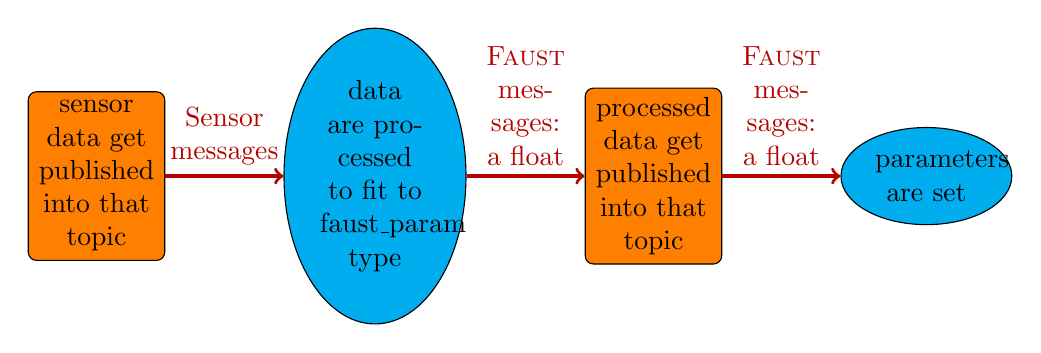
\begin{tikzpicture}[node distance=1.5cm]
	\node[draw, fill=orange, rounded corners=3pt, text width=1.5cm, align=center](sensor topic){sensor data get published into that topic};
	\node[draw, fill=cyan, ellipse, text width=1.4cm, right=of sensor topic, align=center](processing){data are processed to fit to faust\_param type};
	\node[draw, fill=orange, rounded corners=3pt, text width=1.5cm, right=of processing, align=center](faust topic){processed data get published into that topic};
	\node[draw, fill=cyan, ellipse, text width=1.3cm, right=of faust topic, align=center](faust node){parameters are set};
	
	\draw[yoheader,->, very thick] (sensor topic) to node [sloped, midway, above, text width=1.5cm, align=center] {Sensor messages} (processing);
	\draw[yoheader,->, very thick] (processing) to node [sloped, midway, above, text width=1.4cm, align=center] {\faust messages: \\ a float} (faust topic);
	\draw[yoheader,->, very thick] (faust topic) to node [sloped, midway, above, text width=1.4cm, align=center] {\faust messages: \\ a float} (faust node);
\end{tikzpicture}
\caption{Diagram explaining messages dynamic between a sensor topic and a \faust node}
\label{fig:msgs diagram}
\end{figure}\\
Data coming from a sensor need to get processed to be used by a \faust node. For example, if the data is an image message, coming from a camera, you cannot use it directly : you need to perform some processing on the picture, in order t get the value you're interested in. Once this value is processed, you can send it to a \faust topic, on which a \faust node has subscribed. The \faust node is now able to change its parameter value.
\chapter{Common Error Messages}
\label{chap:errors}
Compiling can fail. Here are some common mistakes and how to solve them.
\section{The command does not output anything}
If, after typing your command followed by a file name, your terminal does not output anything like \lstinline'myfile.zip;' or \lstinline'myfile.cpp;' and returns only a blank line, make sure \textbf{you are in the correct directory or you entered the correct path to reach the DSP file.} 

\section{No such file or directory}
If you used the \lstinline'-install' option, make sure you typed the complete workspace path.
For instance, instead of typing this :
\begin{lstlisting}
faust2ros -install myworkspace ~/path/to/myfile.dsp
\end{lstlisting}
you should type :
\begin{lstlisting}
faust2ros -install path/to/myworkspace ~/path/to/myfile.dsp
\end{lstlisting}

\section{Fatal error during \lstinline'catkin_make' operation}
Once your DSP file compiled into a cpp file, if you try to compile it into a \ros executable, the terminal might output :
\begin{lstlisting}
fatal error: faust_msgs/faust_param.h: No such file or directory
\end{lstlisting}
\newpage
You have two possibilities :

\begin{itemize}[leftmargin=*]
	\item If your workspace is only a test workspace, then type :
	\begin{lstlisting}
source path/to/myworkspace/devel/setup.bash
	\end{lstlisting}
	in your terminal.
	\item If your workspace is going to be your current \ros workspace, you can add it to the source directories :
	\begin{lstlisting}
echo "source path/to/myworkspace/devel/setup.bash" >> ~/.bashrc 
	\end{lstlisting}
\end{itemize}

\section{[rosrun] error}
\label{sec:rosrun error}
If, while trying to run a \faust node (called \textit{myname}), an error message showed up saying :

\begin{lstlisting}
[rosrun] Couldn't find executable named myname below /path/to/myworkspace/src/myname
\end{lstlisting}

Then you have to source your workspace :
\begin{itemize}[leftmargin=*]
	\item If your workspace is only a test workspace, then type :
	\begin{lstlisting}
source path/to/myworkspace/devel/setup.bash
	\end{lstlisting}
	in your terminal.
	\item If your workspace is going to be your current \ros workspace, you can add it to the source directories :
	\begin{lstlisting}
echo "source path/to/myworkspace/devel/setup.bash" >> ~/.bashrc 
	\end{lstlisting}
\end{itemize}

\chapter{Cheat Sheet}
\label{cheatsheet}

\section*{Compilation}
\begin{tabular}{p{2cm} p{7cm}}
\lstinline'faust2ros' & compile a .dsp file\\
\lstinline'faust2rosgtk' & compile a .dsp file with a GTK graphic interface\\
\end{tabular}

\paragraph{Options}~\\
\begin{tabular}{p{2cm} p{7cm}}
\lstinline'-install' & installation in a specified workspace\\
\lstinline'-o' & rename the executable\\
\end{tabular}

\paragraph{Example}~\\
\lstinline'faust2ros -install ~/catkin_ws -o harpe4ros ~/dsp/harpe.dsp'


\section*{Run}
\begin{tabular}{p{5cm} p{7cm}}
\lstinline'rosrun harpe4ros harpe4ros' & run the executable \textit{harpe4ros}\\
\end{tabular}
\section*{Metadata}

\lstinline'[ros:/my/topic msg_type msg_name msg_field]'\newline
\lstinline'[ros:/my/topic msg_type msg_name msg_field min_value max_value]'
\chapter{Tutorials}
\label{chap:tuto}
This tutorial will teach you how to use \faust with \ros through the turtlesim package.

\section{DSP File}
Copy the following code into a text file and save it as \lstinline'roscillator.dsp'.

\begin{lstlisting}
declare name 		"roscillator";
declare version 	"1.0";
declare author 		"Grame";
declare license 	"BSD";
declare copyright 	"(c)GRAME 2009";

//-----------------------------------------------
// 			Sinusoidal Oscillator
//-----------------------------------------------

import("music.lib");

smooth(c) = *(1-c) : +~*(c);
vol = hslider("volume [unit:dB][ros:/turtle1/pose turtlesim Pose x 0.0 11.0]", 0, -96, -96, 0.1) : db2linear : smooth(0.999) ;
freq = hslider("freq [unit:Hz][ros:/turtle1/pose turtlesim Pose y 0.0 11.0]", 1000, 20, 24000, 1);


process = vgroup("Oscillator", osc(freq) * vol);

\end{lstlisting}

\newpage

\section{Compilation}
\subsection{If you installed FAUST on your machine}
In a terminal, type :
\begin{lstlisting}
faust2rosgtk -install ~/catkin_ws ~/path/to/roscillator.dsp
\end{lstlisting}
The compilation can take between 10 and 15 seconds.
Then, go in your workspace's root and source the setup file (see section \ref{sec:rostips})

\subsection{With FaustLive}
FaustLive is available on \href{https://sourceforge.net/projects/faudiostream/files/}
{Source Forge}. Once FaustLive installed, launch it.\\
Choose \texttt{Open your File.dsp} and select \texttt{roscillator.dsp}. The file 
will be compiled and executed. 
To export it, clic on \texttt{Window/Export As...} or press \texttt{Ctrl+P}. The Export 
Manager window should be opened.

\begin{figure}[ht!]
\centering
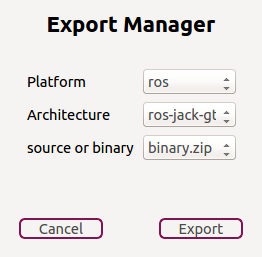
\includegraphics[scale=0.5]{images/faustlive-export.png}
\caption{FaustLive Export Manager}
\label{fig:welcomefaustlive}
\end{figure}

Select \texttt{ros} as platform, \texttt{ros-jack-gtk} as architecture, and \texttt{binary.zip} 
as binary. Then click on \texttt{Export}, and \texttt{Save}. \\
Unzip your package in your current \ros workspace, and make your workspace with 
\texttt{catkin\_make}, and source it (see the \ros tips in section \ref{sec:rostips}).

%\begin{figure}[ht!]
%\centering
%\includegraphics[scale=0.2]{images/faustlive-welcome.png}
%\caption{FaustLive interface}
%\label{fig:welcomefaustlive}
%\end{figure}

\subsection{With the online compiler}
The online compiler is available on \href{http://faust.grame.fr/index.php/online-examples}{the 
\faust Website}. In \texttt{Faust Code} tab, drop your roscillator.dsp file.  In the 
\texttt{Exec File} tab, choose \texttt{Ros ros-jack-gtk} as architecture, and click on 
\texttt{Download the executable file}.\\
Unzip your package in your current \ros workspace, make your workspace with 
\texttt{catkin\_make}, and source it (see the \ros tips in section \ref{sec:rostips}).

\newpage

\section{Run}
In a terminal, run the master : 
\begin{lstlisting}
roscore
\end{lstlisting}
In two new terminals, run the turtlesim node and the teleop\_key node :
\begin{lstlisting}
rosrun turtlesim turtlesim_node
\end{lstlisting}
\begin{lstlisting}
rosrun turtlesim turtle_teleop_key
\end{lstlisting}
In a fourth (and last) terminal, run your \faust node :
\begin{lstlisting}
rosrun roscillator_gtk roscillator_gtk
\end{lstlisting}
You should have four open terminals, a turtle window, and a \faust window.

\begin{figure}[ht!]
\centering
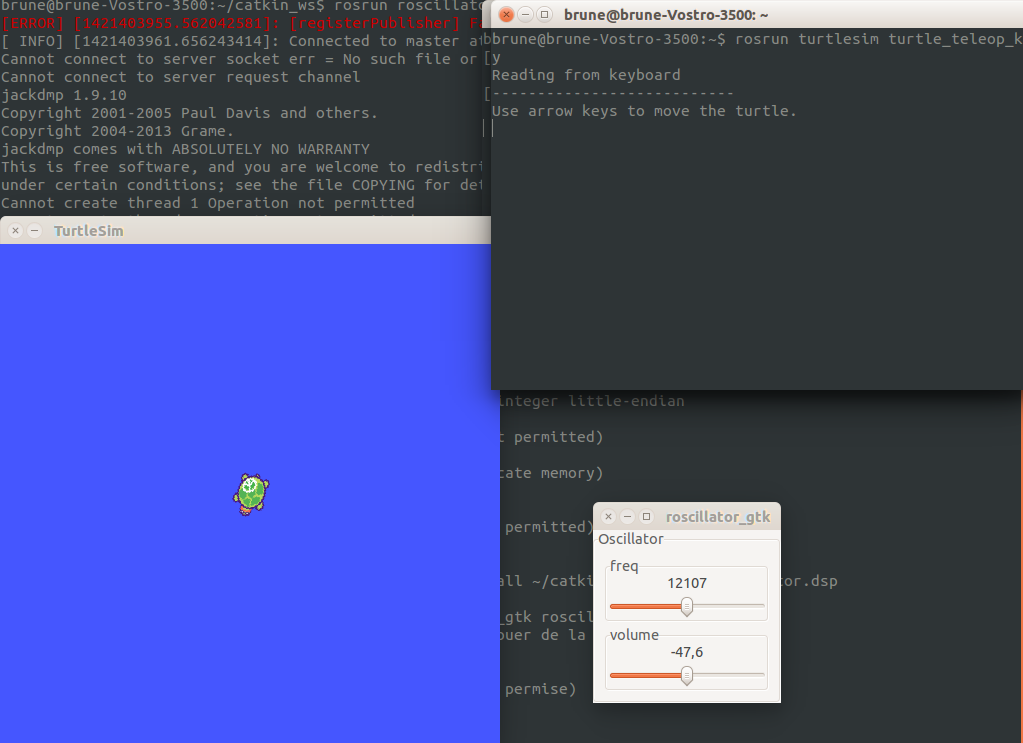
\includegraphics[scale=0.2]{images/tutocommandline.png}
\caption{Screenshot with the four open terminals}
\label{fig:screenshot}
\end{figure}

\subsection{Use}
To move your turtle, go back on the teleop\_key terminal and use your arrow keys.

\newpage

\section{ROS tips}
\label{sec:rostips}
\subsection{How to create a ROS workspace ?} 
\begin{lstlisting}
mkdir -p ~/catkin_ws/src
cd ~/catkin_ws/src
catkin_init_workspace
\end{lstlisting}
\subsection{How to make your workspace ?}
\begin{lstlisting}
cd ~/catkin_ws
catkin_make
\end{lstlisting}
\subsection{How to source a workspace ?}
\begin{lstlisting}
cd ~/catkin_ws
source devel/setup.bash
\end{lstlisting}

\end{document}
